%!TEX root = these.tex

\begin{appendices}
% \appendixpage
\clearpage
\let\clearpage\relax
\vspace*{\fill}
\begin{center}
  \Huge\bfseries Annexe
\end{center}

\vspace*{\fill}
% \noappendicestocpagenum
% \addappheadtotoc
\chapter{Annexe}
\label{appendix:annexe}
\section{Notions clefs de biologie structurale}
	Cette section définit et détaille les notions clefs de biologie structurale abordées au cours du chapitre~\ref{chap2}.
	
	\subsection{Liaisons covalentes}
	Une liaison covalente est une liaison chimique dans laquelle deux atomes partagent deux électrons (un électron chacun ou deux électrons venant du même atome) d'une de leurs couches externes afin de former un doublet d'électrons liant les deux atomes. C'est une des forces qui produit l'attraction mutuelle entre atomes.
	
	La liaison covalente implique généralement le partage équitable d'une seule paire d'électrons, appelé doublet liant. Chaque atome fournissant un électron, la paire d'électrons est délocalisée entre les deux atomes. Le partage de deux ou trois paires d'électrons s'appelle respectivement \og liaison double \fg{} et \og liaison triple \fg{}.
	
	Au contraire des liaisons ioniques où les atomes sont liés par attraction coulombienne non-directionnelle, les liaisons covalentes sont fortement directionnelles. En conséquence, les molécules liées par covalence tendent à adopter des formes caractéristiques possédant des angles de liaison spécifiques.
	
	\FloatBarrier \subsection{Protéines}
	Les protéines sont des macromolécules\footnote{Une macromolécule est une \og grosse \fg{} molécule, généralement un polymère ; elle est constituée de plusieurs milliers d'atomes.} que l'on retrouve dans les cellules de tous les organismes vivants. Elles assurent un très grand nombre de fonctions cellulaires (structuration de la cellule, mouvements et divisions cellulaires, communication intercellulaire, transport, par exemple de dioxygène, défense immunitaire) et biochimiques (liaison et fixations de molécules, catalyse de réactions biochimiques, etc.) au sein des cellules et des tissus~\cite{lodish2004molecular}. Elles participent aussi au conditionnement de l'acide désoxyribonucléique (ADN) et à la régulation de l'expression génétique. L'étude de leur fonctionnement est donc essentiel à la compréhension du vivant et de ses processus.
	
	\begin{wrapfigure}{O}{0.5\textwidth} % Capital O makes the figure float, because that's totally intuitive and obvious.
		\centering
		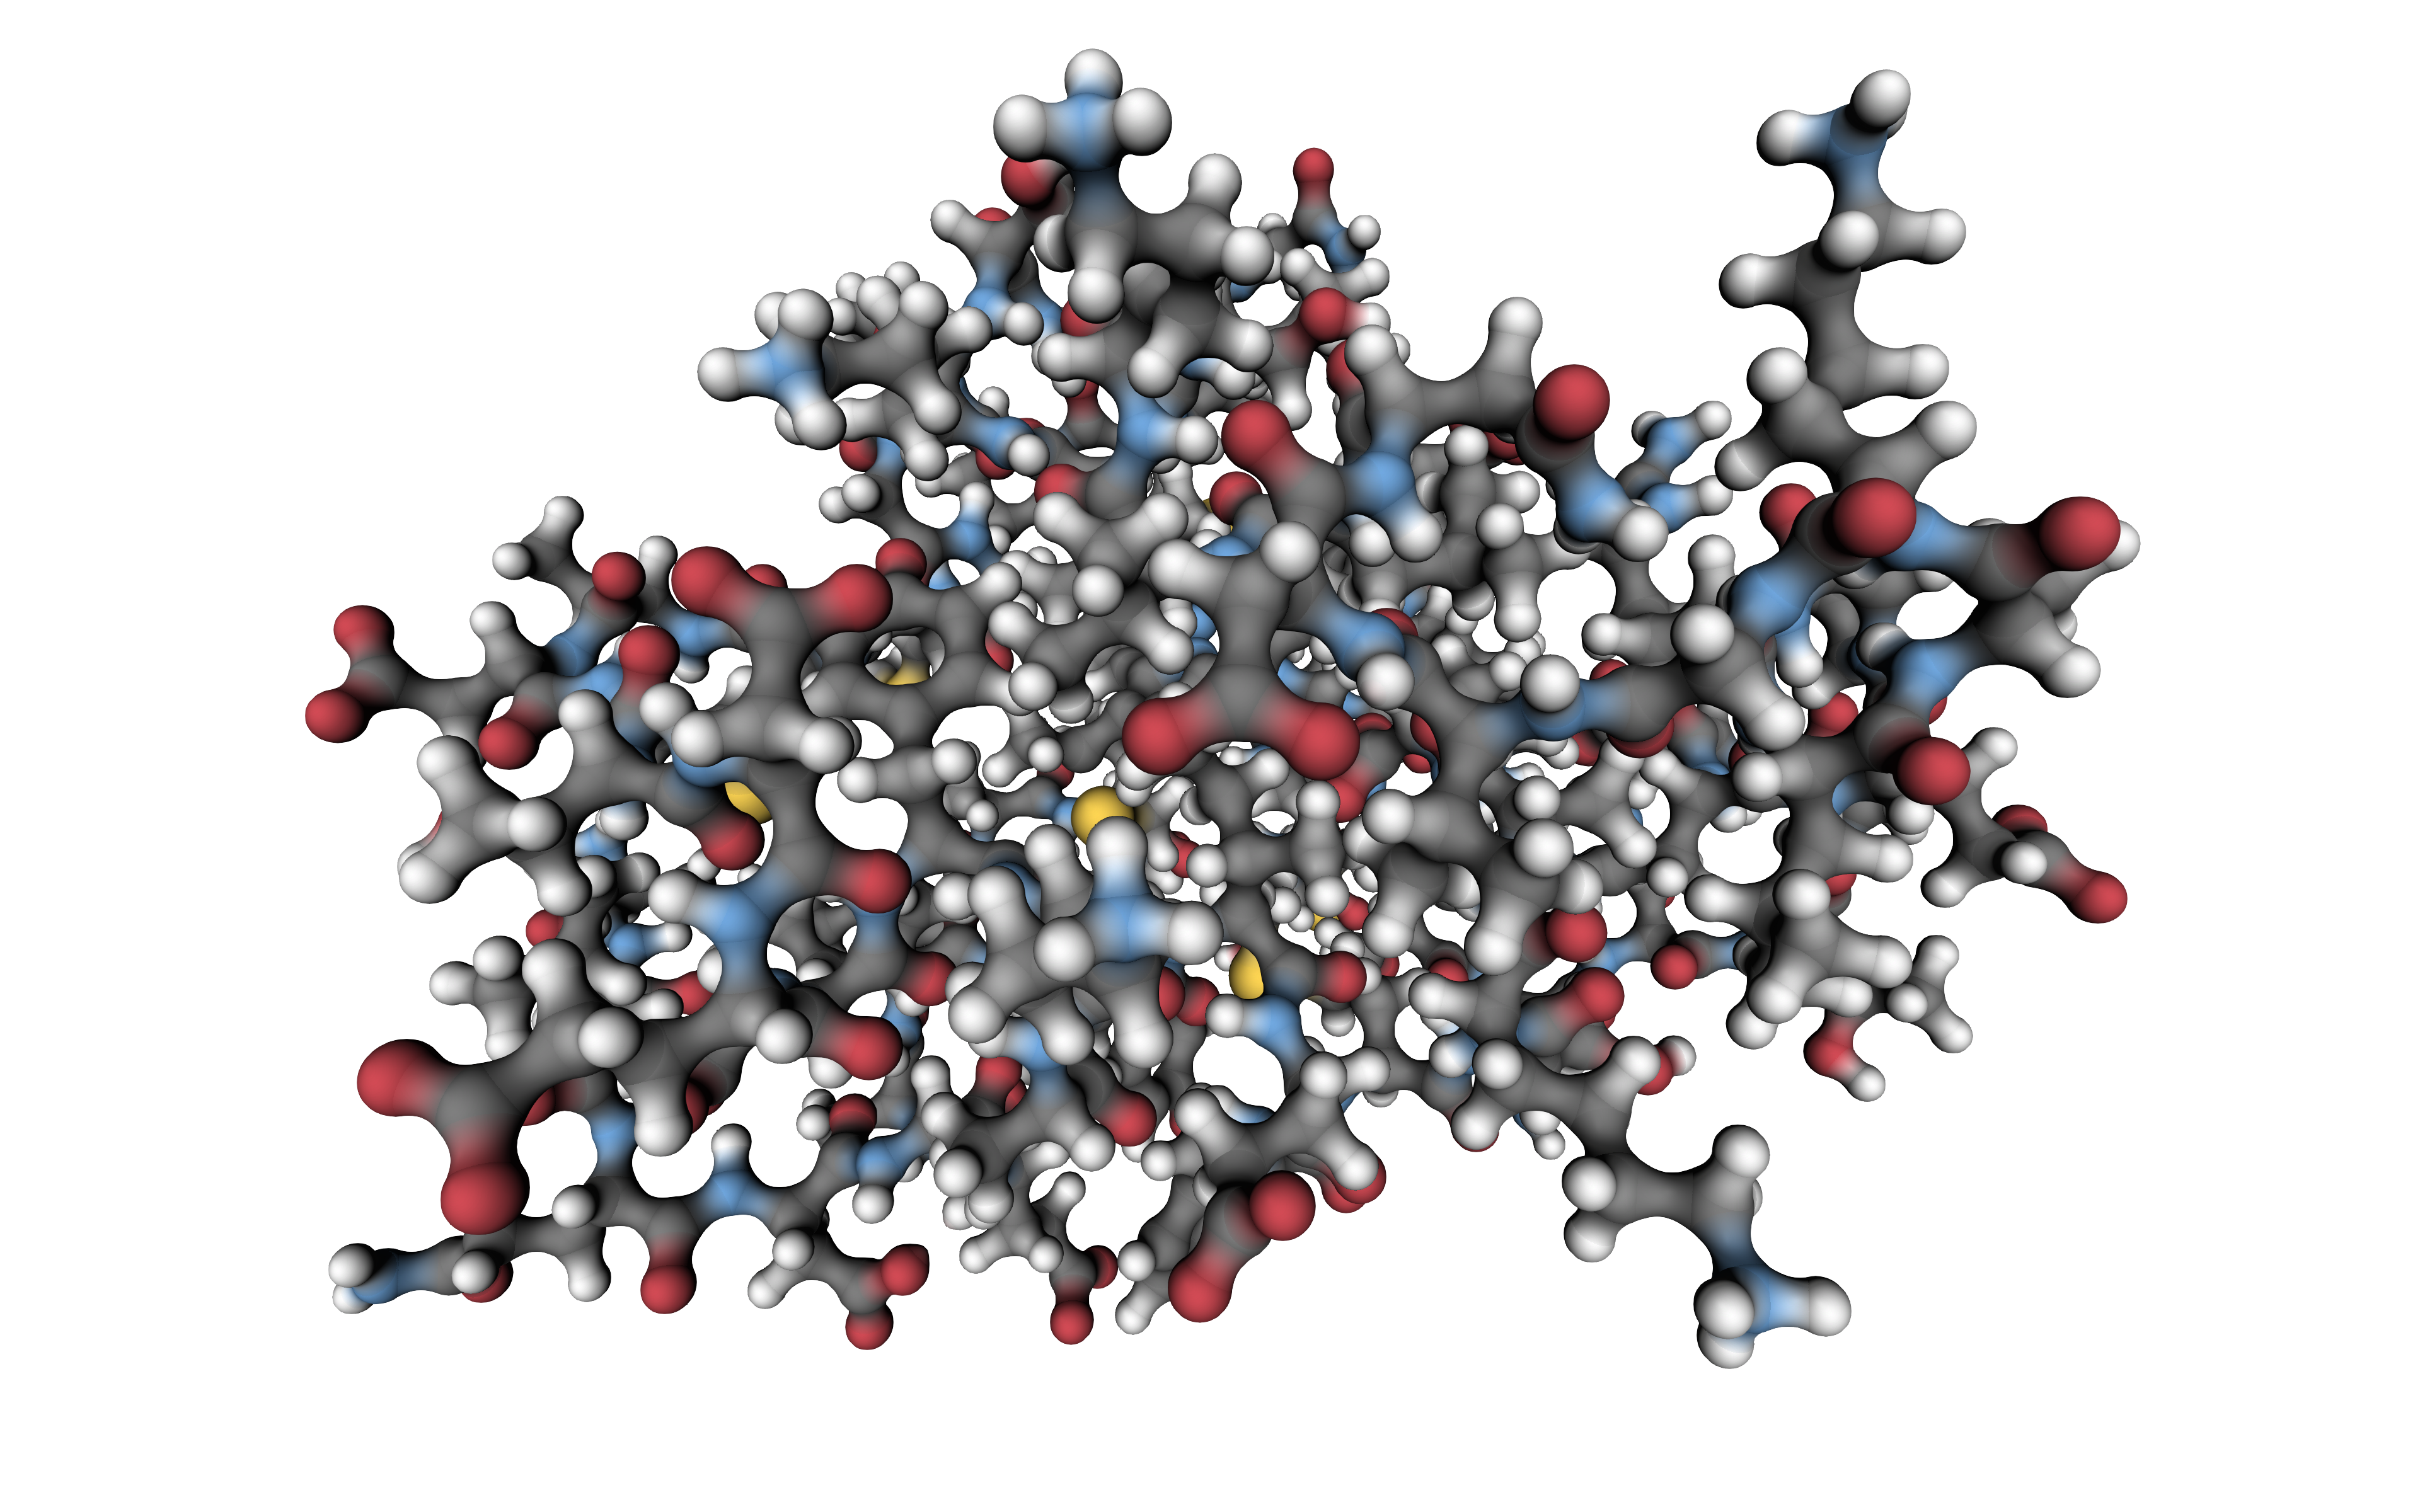
\includegraphics[width=0.46\textwidth]{figures/ch1/1KX2}
		\caption[Une protéine en \emph{Hyperballs}]{Une protéine (\cite{bartalesi2002solution}) représentée avec UnityMol~\cite{doutreligne2014unitymol}. Elle est assez petite (81 acides aminés, vs. $\approx$~30~000 pour la titine), les atomes sont représentés avec un rayon inférieur à leur rayon de vdW, l'occultation est réduite, et les molécules du solvant ne sont pas représentées. Malgré tout, le niveau d'occultation demeure très important.}
		\label{fig:1KX2}
	\end{wrapfigure}
	
	\subsubsection{Composition}
	Concrètement, une protéine est un une chaîne d'acides aminés, reliés par des liaisons peptidiques, c'est-à-dire des liaisons covalentes entre une fonction carboxyle (–C(O)OH) et une fonction amine (un composé organique dérivé de l'ammoniac dont au moins un atome d'hydrogène a été remplacé par un groupe carboné). Ces chaînes d'acides aminés sont également appelées chaînes polypeptidiques, ou simplement polypeptides.
	
	\subsubsection{Synthèse}
	Un gène est un brin d'ADN qui \og code \fg{}  une protéine. Dans la cellule, ce brin d'ADN, composé de quatre nucléotides différents : adénine, cytosine, guanine et thymine (A, C, G, T) subit une \emph{transcription} en un brin d'ARN messager, composé également d'adénine, cytosine et guanine, mais d'uracil à la place de la thymine (A, C, G, U). Par exemple, la séquence \texttt{TAGTTCCAGTCAGT} serait transcrite en \texttt{UAGUUCCAGUCAGU}. Si l'ADN a pour fonction de stocker l'information génétique, l'ARN messager permet, comme son nom l'indique, de la communiquer au ribosome, un complexe moléculaire chargé de l'étape de \emph{traduction}.
	
	La traduction se fait selon le \emph{code génétique} illustré par la figure~\ref{fig:geneCode}. Ainsi, à chaque \emph{codon} (non-stop) est associé un acide aminé.
	
	\begin{figure}[htb]
		%\centering
		\begin{subfigure}[t]{0.44\textwidth}
			\centering
			\includegraphics[width=\textwidth]{figures/ch1/geneCode}
			\caption[Le code génétique]{Ce diagramme illustre la correspondance entre un \emph{codon}, c'est-à-dire une suite de trois nucléotides (par exemple \texttt{UCG}) et l'acide aminé associé (dans le même exemple, la serine). On lit un codon du centre vers la périphérie du diagramme. Crédit : J\_{}Alves\footnotemark{}.}
			\label{fig:geneCode}
		\end{subfigure}
		~
		\begin{subfigure}[t]{0.54\textwidth}
			\includegraphics[width=\textwidth]{figures/ch1/translation}
			\caption[Traduction de l'ARN messager en protéine]{Traduction de l'ARN messager et synthèse d'une chaîne polypeptidique. Des ARN de transfert apportent les acides aminés au ribosome qui, en les liant aux bons codons sur le brin d'ARN messager, construit la chaîne polypeptidique dont la protéine finale sera constituée. Crédit : Liberty Voice\footnotemark{}.}
			\label{fig:translation}
		\end{subfigure}
		\label{fig:codeTrans}
		\caption{Code génétique et traduction.}
	\end{figure}
	
	\addtocounter{footnote}{-1}
	\footnotetext{\url{https://openclipart.org/detail/95203/genetic-code-rna}}
	\addtocounter{footnote}{1}
	\footnotetext{\url{http://guardianlv.com/2013/10/naked-mole-rat-longevity-explained-by-higher-translational-fidelity}}
	
	Le ribosome peut ainsi synthétiser une protéine à partir d'un brin d'ARN messager en associant le bon acide aminé à chaque codon, comme l'illustre le montre la figure
	
	\subsubsection{Structure}
	Les protéines sont décrites selon plusieurs niveaux de structures. On appelle structure primaire, la suite d'acides aminés qui composent la protéine, résultat de la traduction séquentielle d'un gène de l'ADN en protéine selon les règles du code génétique universel, dans lequel à chacun des 64 triplets possibles de nucléotides (A,C,G,T) composant l'ADN, correspond à un acide aminé. À ce niveau de structure, c'est la séquence qui est importante, la protéine étant considérée comme un collier de perles, chaque perle étant un des 22 acides aminées.
	
	Ensuite, pendant et après la synthèse, les protéines s'organisent en 3D pour former des architectures typiques, et cette organisation correspond à la structure secondaire~\cite{foltmann1981protein} qui est en fait une description de la structure tridimensionnelle localement adoptée par un segment de molécule. Cette structure secondaire s'explique par les liaisons hydrogène qui connectent et rapprochent spatialement certains segments, plus précisément entre les groupements amide et carbonyle du squelette peptidique, dans le cas des protéines, et entre les bases nucléiques dans le cas des acides nucléiques (acide désoxyribonucléique, ou ADN, et acide ribonucléique, ou ARN). Parfois, cette définition est assouplie et un segment peut être considéré comme une structure secondaire particulière sur la base des valeurs de certains de ses angles dièdres, indépendamment des liaisons hydrogène. Les algorithmes couramment utilisés pour identifier les structures secondaires incluent DSSP~\cite{kabsch1983dictionary}, \emph{Define}~\cite{richards1988identification}, \emph{Stride}~\cite{frishman1995knowledge} et SST~\cite{konagurthu2012minimum}.
		
	Dans la majorité des cas, une structure secondaire est soit une hélice alpha, soit un feuillet bêta~\cite{pauling1951structure}, soit un segment sans architecture ni contrainte appelé boucle. Dans une représentation dite \og en structures secondaires \fg{} ces segments de molécule sont remplacés par des représentations plus schématiques. Un exemple pour une hélice alpha est présenté dans la figure~\ref{fig:aHelix}, et un exemple pour un feuillet bêta est fourni sur la figure~\ref{fig:bSheet}. L'utilisation de ces schématisations permet de considérablement simplifier la représentation de la molécule finale, comme l'illustre la figure~\ref{fig:4awn_ss}.
	
	\begin{figure}[H]
		%\centering
		\begin{subfigure}[b]{.49\textwidth}
			\centering
			\includegraphics[width=\textwidth]{./figures/ch1/aHelix}
			\caption[Hélices alpha, trois représentations différentes]{Une hélice alpha schématisée (gauche), avec du texte représentant les atomes (centre) et en représentation \og tout atome \fg{} (droite). Lors d'un affichage \og en structures secondaires \fg{} la représentation de gauche est plus courante. Crédit : \emph{Bioinformatics -- An Introduction}, Bioinformatics Lab, AU\footnotemark.}
			\label{fig:aHelix}
		\end{subfigure}
		~
		\begin{subfigure}[b]{.49\textwidth}
			\centering
			\includegraphics[width=\textwidth]{./figures/ch1/bSheet}
			\caption[Feuillets bêta]{Un feuillet bêta en représentation \og tout atome \fg{} (à gauche), sous forme schématique (au milieu), et en représentation \og tout atome \fg{} mixte (à droite). Lors d'un affichage \og en structures secondaires \fg{} la représentation du milieu est généralement choisie. Crédit : \emph{Department of Biology} -- PSU\footnotemark.}
			\label{fig:bSheet}
		\end{subfigure}
		\caption{Structures secondaires.}
		\label{fig:secStructs}
	\end{figure}
	
	\addtocounter{footnote}{-1}
	\footnotetext{\url{http://bioinfo.au-kbc.org.in/books/bi/1.html}}
	\addtocounter{footnote}{1}
	\footnotetext{\url{https://wikispaces.psu.edu/display/Biol230WCE/Properties+of+Macromolecules+I-Proteins}}
		
	De plus, ces représentations schématiques correspondent à des critères physiques ou chimiques précis et pertinents pour l'analyse des molécules concernées. La représentation en structures secondaires permet donc de simplifier la représentation tout en communicant efficacement des informations précises sur la molécule affichée~\cite{richardson2002teaching}. La molécule devient plus facile à observer, et sa structure est plus lisible.
		
	Toutefois, l'utilisation de cette technique de visualisation implique une perte d'information. En effet, les atomes ne sont plus visibles, aussi la composition précise de la molécule n'est-elle plus perceptible. De fait, il devient difficile d'apprécier certaines propriétés physico-chimiques du système.

	Dans la littérature anglo-saxonne, la représentation en structures secondaires est parfois appelée \emph{cartoon} ou \emph{ribbons}~\cite{carson1986algorithm, richardson2000early}.
	
	\subsubsection{Rôles}
	Les protéines sont impliquées dans la plupart des processus biologiques et, de fait, leurs rôles sont extrêmement divers. On peut toutefois les diviser en deux grandes parties : les fonctions cellulaires et les fonctions biochimiques. Les premières définissent le rôle de la protéine dans la cellule ou l'organisme, et peuvent être découpées en cinq groupes~\cite{lodish1995molecular} :
	\begin{enumerate}
		\item Les protéines des structures, qui permettent à la cellule de maintenir son intégrité physique et son organisation dans l'espace. C'est par exemple la fonction du collagène, la protéine la plus abondante chez les mammifères~\cite{di2002mapping}.
		\item Les protéines de transport, qui acheminent les molécules nécessaires aux fonctions cellulaires au sein des cellules, mais aussi à travers les membranes nucléaires et plasmiques, ou hors des cellules. Cela inclut notamment le transport de dioxygène par l'hémoglobine, de fer par la transferrine~\cite{crichton1987iron} ou d'ions à travers les membranes cellulaires, par les canaux ioniques. 
		\item Les protéines régulatrices, qui inhibent ou stimulent l'activité d'autres protéines, ou la transcription de gènes, ce qui permet réguler divers processus biologiques.
		\item Les protéines de signalisation, qui reçoivent les signaux extérieurs (en se liant aux molécules qui les transmettent ou en réagissant à leur contact) et assurent leur transmission vers la cellule, ou vers une autre zone de l'organisme. Les protéines de signalisation permettent notamment de réagir aux hormones ; lorsque celles-ci sont hydrophiles (et donc incapables de traverser la membrane cellulaire, composée de lipides), les protéines réceptrices sont transmembranaires, leur extrémité extérieure permet la fixation de l'hormone, tandis que l'extrémité intérieure transmet le signal. C'est notamment le cas des récepteurs de l'insuline~\cite{gammeltoft1984insulin}. Lorsque les hormones sont lipophiles et peuvent traverser la membrane, la protéine réagit à la fixation de l'hormone par un changement conformationnel qui lui permettra de transmettre le signal. 
		\item Les protéines motrices, qui permettent aux cellules ou aux organismes de se mouvoir. On peut citer par exemple la myosine, essentielle à l'activité musculaire des vertébrés~\cite{pollard1973acanthamoeba}.
	\end{enumerate}	
	
	
	\subsection{Ligands}
	Un ligand est une molécule qui se lie de manière réversible sur une macromolécule ciblée, protéine ou acide nucléique, jouant en général un rôle fonctionnel : stabilisation structurale, catalyse, modulation d'une activité enzymatique, transmission d'un signal. Par exemple, le hème de la myoglobine est un ligand, cf. la figure~\ref{fig:myoglobin}.

\section{Annotations de vidéos, données complémentaires}

	\begin{figure}[!htb]
		\begin{subfigure}[t]{\subImgWclicks}
			\centering
			\includegraphics[width=\textwidth]{figures/annexe/bulletA_filteredSpeed}
			\caption{Vitesses.}
			\label{fig:bulletA_filteredSpeed}
		\end{subfigure}
		~
		\begin{subfigure}[t]{\subImgWclicks}
			\centering
			\includegraphics[width=\textwidth]{figures/annexe/bulletA_frequency}
			\caption{Fréquences.}
			\label{fig:bulletA_frequency}
		\end{subfigure}
		~
		\begin{subfigure}[t]{\subImgWclicks}
			\centering
			\includegraphics[width=\textwidth]{figures/annexe/bulletA_angle}
			\caption{Angles.}
			\label{fig:bulletA_angle}
		\end{subfigure}
		\caption[Histogrammes pour la balle de pistolet]{Histogrammes pour la balle de pistolet.}
		\label{fig:histBullet}
	\end{figure}
	
\begin{table}
	\centering
	\begin{tabular}{c c c c c c c c c}
		$V_{max}$	& $\overline{V}$	& $\sigma_{V}$	& $F_{max}$	& $\overline{F}$	& $\sigma_{F}$	& $A_{max}$	& $\overline{A}$	& $\sigma_{A}$	\bigstrut[b] \\ \hline

		105,45		& 10,27				& 15,96			& 30,00		& 18,24				& 10,41			& 175,06	& 45,23				& 47,83			\bigstrut[t] \\
	\end{tabular}
	\caption[Statistiques pour la vidéo de balle de pistolet]{Statistiques pour la vidéo de balle de pistolet.}
	\label{tab:bulletA_stats}
\end{table}



%\chapter{Annexe B}
%\label{appendix:annexeB}




\end{appendices}